%IMPORTS
\documentclass[a4paper, 11pt]{article}
\usepackage[utf8]{inputenc} 
\usepackage[T1]{fontenc}
\usepackage[catalan]{babel}
\usepackage{amsmath, amssymb, amsthm}
\usepackage[margin=1in]{geometry}
\usepackage{enumerate}
\usepackage{array}
\usepackage{graphicx}
\usepackage{wrapfig}
\usepackage{ragged2e} 
\usepackage{subfig}
\usepackage{caption}
\usepackage{subcaption}
\usepackage[dvipsnames]{xcolor}
%\usepackage[table]{xcolor}
\usepackage{float}
\usepackage{chngcntr}
\usepackage{ragged2e}
\usepackage{multirow}
\usepackage{vmargin}
\usepackage{hyperref}
\usepackage{url}
\usepackage{fancyhdr}
\usepackage{bigints}
\usepackage{listings}
\usepackage{xcolor,colortbl}
\usepackage{longtable}
\usepackage{verbatim}
\usepackage{xcolor, colortbl}
\usepackage{array, multirow, multicol}

\definecolor{lightapricot}{rgb}{0.99, 0.84, 0.69}
\definecolor{lavenderblue}{rgb}{0.8, 0.8, 1.0}
\definecolor{navy}{rgb}{0,0,128}
\definecolor{codegreen}{rgb}{0,0.6,0}
\definecolor{codegray}{rgb}{0.5,0.5,0.5}
\definecolor{codepurple}{rgb}{0.58,0,0.82}
\definecolor{backcolour}{rgb}{0.95,0.95,0.92}
\definecolor{amaranth}{rgb}{0.9, 0.17, 0.31}
\definecolor{GRAY}{rgb}{0.75, 0.75, 0.75}
\definecolor{deepfuchsia}{rgb}{0.76, 0.33, 0.76}
\definecolor{deepmagenta}{rgb}{0.8, 0.0, 0.8}
\definecolor{funcblue}{rgb}{0.36, 0.57, 0.9}


\begin{document}
\begin{titlepage}
    \centering
    {\bfseries\LARGE \hspace{1.9em} Universitat Autònoma de Barcelona\newline Facultat de Ciències\par}
    \vspace{2cm}
    {\hspace{-1em}
\includegraphics[width=0.6\textwidth]{MatCAD3.jpg}\par}
    \vspace{1cm}
    {\scshape\Huge Cas Kaggle: \par Classificació de categories de pel·licules i series de Netflix\par} 
    \vspace{1cm}
    {\Large \itshape Autor: \par}
    \vspace{0.5cm}
    {\Large Gerard Lahuerta \par}
    \vspace{0.5cm}
    {\Large 1601350 \par}
    \vspace{1cm}
    {\Large 16 de Desembre del 2022 \par}
\end{titlepage}

\justifying

\newpage
{
\small
\setcounter{page}{2}
\pagestyle{plain}
\tableofcontents
\cleardoublepage
\addcontentsline{}{chapter}{}
}
\newpage
\section{Introducció}
\subsection{Presentació del treball}
L'objectiu d'aquesta pràctica és, mitjançant la interfície proporcionada per Jupyter Notebook, estudiar i classificar una serie o pl·licula de l'empressa Netflix segons el seu rang de classificacions\footnote{El rang de classificació de les series i pel·licules esta explicat a l'aprtat \textcolor{blue}{\ref{exp_dataset}}}. \\
Les dades han sigut proporcionades per la web de Kaggle, concretament, la base de dades de series i pel·licules de Netflix.\\\\
El dataset que s'utilitza es pot trobar al següent enllaç:
\begin{center}
    \text{\small\textcolor{blue}{\url{https://www.kaggle.com/shivamb/netflix-shows}}}.
\end{center}
\newpage
\subsection{Llibreries i importacions}
Per tal de poder dur a terme aquesta tasca és imprescindible tenir intal·lades les següents llibreries, ja que s'utilitzen les funcions següents (d'entre altres).

\begin{table}[h]
    \centering
    \begin{tabular}{c|c}
        \textbf{Llibreria} & \textbf{Funció utilitzada} \\\hline\hline
        sklearn.datasets & make\_regression \\ \hline
         \multirow{2}{*}{pandas (as pd)} & read\_csv \\ 
        & DataFrame \\ \hline
        \multirow{4}{*}{matplotlib pyplot (as plt)} & figure\\
        & plot \\ 
        & hist \\
        & scatter\\ \hline
        seaborn (as sns) & heatmap \\\hline
        \multirow{2}{*}{sklearn.linear\_model} & LogisticRegression \\
         & LogisticRegressionCV \\\hline
        sklearn.tree & DecisionTreeClassifier\\ \hline
        \multirow{7}{*}{sklearn.metrics} & confusion\_matrix \\ 
        & ConfusionMatrixDisplay \\
        & precision\_recall\_curve\\
        & average\_precision\_score\\
        & roc\_curve\\
        & auc \\
        & precision\_score \\\hline
        \multirow{3}{*}{sklearn.model\_selection} & cross\_val\_score \\ 
        & cross\_validate \\
        & train\_test\_split \\\hline
        sklearn.ensemble & RandomForestClassifier \\\hline
        sklearn.neighbors & KNeighborsClassifier \\ \hline
        sklearn.pipeline & make\_pipeline\\ \hline
        sklearn.preprocessing & StandardScaler\\ \hline
        \multirow{2}{*}{sklearn.svm} & SVC\\ 
        & LinearSVC \\\hline
        sklearn.cluster & KMeans \\\hline
        sklearn.mixture & GaussianMixture \\ \hline
        warnings & filterwarnings \\ \hline
        \multirow{2}{*}{numpy (as np)} & meshgrid \\
        & concatenate \\
    \end{tabular}
    \label{imports}
    \caption{Llibreries i funcions utilitzades}
\end{table}
\subsection{Criteris i assumcions}
S'han tingut en compte els següents criteris per a la correcta classificació de les dades:
\begin{enumerate}
    \item Degut a la gran quantitat d'informació que s'obté en el proces de tractament de les dades; només s'utilitzarà amb les més rellevant.
    \item Es preferible etiquetar un element en una classe que no hi pertany que no etiquetar un element d'una classe a la que hi pertany.
\end{enumerate}

\newpage
\section{Gestió i estudi del Dataset}
\subsection{Explicació del Dataset} \label{exp_dataset}
El dataset tracta sobre les series i pel·licules que hi disposa l'empressa Netflix per al seu consúm. \\
L'objectiu del treball és, mitjançant les dades disposades, poder general models capaços de classificar, mitjançant el minim nombre d'atributs disponibles, les categories a les que pertany les noves series i pel·licules
(apartir d'ara ens referirem a les series i pel·licules com: \textit{producció})  que hi afegeixen en la plataforma.\\\\
El dataset en qüestió té una mida de 8807 x 12 (files x columnes). \\
Els 12 atributs recollits de les produccions són:

\begin{table}[h!]
    \centering
    \begin{tabular}{l|l|l}
        \textbf{Atribut} & \textbf{Explicació} & \textbf{Tipus de dada}\\\hline\hline
        type & serie o pel·licula & string\\\hline 
        title & titól de la producció & string\\\hline
        director & nom del director de la producció & string \\\hline
        cast & actors de la producció &  string \\\hline
        country & païs on és grabada la producció & string \\\hline
        data\_added & data quan va ser afegida la producció al catèleg & string\\\hline
        release\_year & any quan va ser estrenada la producció & int  \\\hline
        rating & etiqueta de destinació de la producció (TV/PG) & string \\\hline
        duration & durada de la producció (minuts o temporades) & string \\\hline
        listed\_in & generes de la producció & string \\\hline
        description & synopsis de la producció & string
    \end{tabular}
    \caption{Explicació dels atributs i el seu rang de valors que assoleixen}
    \label{explicació_atributs}
\end{table}
\hspace{-2.1 em}
Cal destacar que la gran majoria d'atributs son de tipus string o llistes d'string; per aquest motius es decideix utilitzar un one-hotter-coding dels atributs de tipus string.\\\\
També, cal mencionar, que part dels atributs poden ser omesos per que de manera lógica és veu que no hi tenen relació entre el genere i el valor de l'atribut (a l'hora de classificar futures produccions que s'incloguin al cataleg) o per la dificultat que hi pot existir per a utilitzar el valor de l'atribut de manera generica per a classificar la producció. Alguns d'aquests atributs que és poden ometre son:
data\_added\footnote{S'observa de manera clara com el any que va ser afegida al cataleg una producció no afecta a quin genere pertany.} i director\footnote{El director (així com el repart de la producció), si bé es pot utilitzar per a classificar la producció ja que molt artistes/directors graben generes semblants, la quantitat de paràmetres que ens generaria el one-hotter-coding per aquests atributs seria tant gran que dificultaria la seva gestió i utilització en la classificació.}. 
\newpage
\subsection{Distribució de les dades}
S'iniciarà  l'estudi del dataset observant la distribució de les dades per intuïr relacions senzilles des d'on començar a plantejar els primers models, així com crivar els atributs rellevants per a fer la classificació.\\\\
Es mostren ara alguns dels histogrames generats, així com \textit{scatter-plots} del \textit{price\_range} respecte les variables. 

\begin{figure}[h]
    \centering
  \subfloat[\textit{Movie Duration}]{
    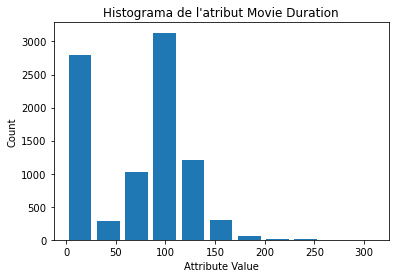
\includegraphics[width=0.3\textwidth]{Histogramas/hist_movieDuration.png}}
  \subfloat[\textit{Release Year}]{
    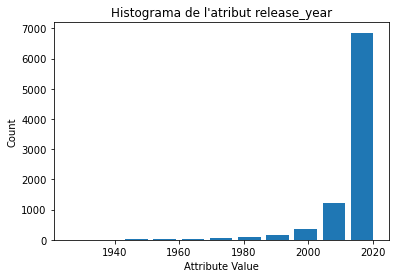
\includegraphics[width=0.3\textwidth]{Histogramas/hist_releaseYear.png}}
  \subfloat[\textit{United State of America}]{
    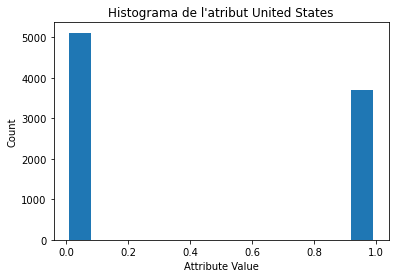
\includegraphics[width=0.3\textwidth]{Histogramas/hist_USA.png}}
    \caption{Mostra dels histogrames generats per l'estudi inicial}
\end{figure}
\hspace{-1.4 em}S'observen les següents característiques dels histogrames\footnote{És pot consultar el conjunt de histogrames al notebook entregat conjuntament amb aquest informe}:
\begin{itemize}
    \item [$\circ$] Degut al one-hotter-coding la majoria d'atributs tenen distribucions binaries.
    \item [$\circ$] S'observa com no hi existeix una uniformitat en el nombre de produccions de diferents generes, sent més populars uns que altres. Degut aquesta no uniformitat, hi pot haber problemes en la classificació dels generes. És discutirà aquest tema més endavant.
\end{itemize}
Per a obtenir millors conclusions, es decideix veure les relacions dels atributs representant els objectius respecte la resta d'atributs. Mostrem ara alguns exemples dels resultats obtinguts
\begin{figure}[h]
    \centering
  \subfloat[Clasic Movies vs Release Year]{
    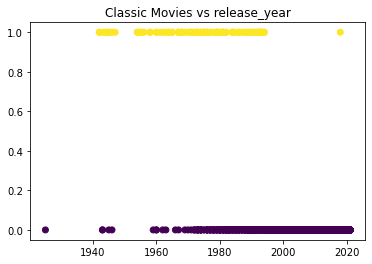
\includegraphics[width=0.3\textwidth]{Scatterplots/ClassicMoviesvsReleasedYear.png}}
  \subfloat[TV Drama vs Seasons]{
    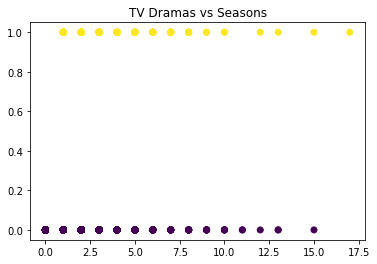
\includegraphics[width=0.3\textwidth]{Scatterplots/DramasvsSeasions.png}}
  \subfloat[Kid's TV vs Movie Duration]{
    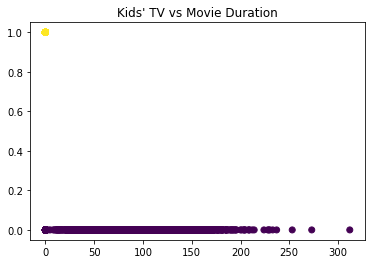
\includegraphics[width=0.3\textwidth]{Scatterplots/kidsvsMovieDuration.png}}
    \caption{Mostra dels \textit{scatter-plots} generats per l'estudi inicial}
\end{figure}\\
\hspace{-1.4 em}És conclou dels \textit{scatter-plots} \footnote{El conjunt sencer d'\textit{scatter-plots} són al notebook entregat conjunt aquesta memória} que no es percep de manera intuïtiva cap relació entre les variables. \\\\
És procedeix a estudiar les correlacions de variables per trobar relacions entre elles i els nostres atributs objectius.
\newpage
\subsection{Correlació de les variables}\label{correlacio}
S'ha decidit estudiar la correlació entre els atributs que conté la base de dades per tal d'analitzar la importància entre ells per poder trobar els millors paràmetres per classificar i decidir com tractar les incongruències de les dades exposades anteriorment a l'apartat \textcolor{blue}{\ref{exp_dataset}}.

\begin{figure}[h] % Flotante "comun", sin caption, en que irán ambos
\begin{minipage}{10cm} % Minipagina para la tabla. 8 cm de ancho
\begin{center}
    \begin{tabular}{l|l|l}
        \textbf{Gènere} & \textbf{Atribut} & \textbf{Correlació}\\\hline\hline
        Documentaries & Seasons & -0.149\\\hline
            \multirow{6}{*}{ International TV Shows} &  Movie Duration  & -0.572 \\
        &Taiwan       &     0.178 \\
        &South Korea   &    0.229 \\
        &Japan        &     0.173 \\
        &United States  &  -0.314 \\
        &Seasons      &     0.312 \\\hline
        \multirow{2}{*}{TV Dramas} & Movie Duration  & -0.414 \\
        & Seasons     &      0.340\\\hline
        \multirow{2}{*}{TV Mysteries} & Movie Duration &   -0.143 \\
 & Seasons       &    0.148\\\hline
        \multirow{5}{*}{Romantic TV Shows} & Movie Duration &   -0.282 \\
& Taiwan        &     0.250 \\
& South Korea   &    0.239 \\
& United States  &  -0.127 \\
& Seasons      &     0.151 \\\hline
        \multirow{5}{*}{Spanish-Language TV Shows} & Movie Duration &  -0.191 \\
& Colombia      &    0.309 \\
& Argentina    &     0.131 \\
& Spain      &       0.186 \\
& Mexico      &      0.260\\\hline
         $\vdots$ & $\vdots$ & $\vdots$
    \end{tabular}
    \label{tab:afins}
    Taula 3: Correlacions d'alguns atributs    \setcounter{table}{3}
\end{center}


\end{minipage} % Fin de la minipagina de la tabla
\hspace{2em}
%\hfill % Espacio flexible para separar tabla y figura
\begin{minipage}{4cm} % Minipágina para la figura, 6 cm de ancho
Mostrem a la taula els atributs que tenen una correlació millor que el $ 70\% $ d'elles; és a dir, $ cor_i \geq \mu + \sigma$ on $\mu$ és ma mitjana de les correlacions per al genere escollit i $\sigma$ la desviació estandard.\\\\
A partir dels resultats obtinguts es pot deduïr que hi existeixen molt poques bones correlacions entre els atributs. \\\\
Per aquest motius és procedira a analitzar visualment les interacions dels atributs més rellevants entre ells i com afecten a l'etiquetatge.

\end{minipage} % Fin de la minipagina que lleva la foto
\end{figure} % Fin del entorno comun. No lleva caption
\hspace{-1.5em}S'observa, mitjançant les dades obtingudes\footnote{És pot consultar la totalitat de les correlacions rellevants en el notebook entregat conjuntamnet amb la memória}, com hi han atributs rellevants per a cert gèneres que en altres no hi son pas. \\\\ Per aquest motius és pot teoritzar que és pot parametritzar diferents models de predicció per a cada gènere i, per tant, podem crear un model que categoritci les produccions mitjançant un conjunt de models diferents per a cada gènere.\\\\
Mencionar, a més, que s'obté atributs que no tenen correlacions significatives, aixó és per la falta de dades de produccions d'aquell tipus; per aquest motius és decideix no treballar amb aquestes dades ja que no s'obtindrà una classificació decent al no tenir la suficient informació com per a testejar i entrenar debidament (i la creació de noves dades mitjançant les que ja és disposa és desestimat degut a que tampoc és disposa amb dades suficients com per a crear un model de regressió amb bones prediccions capaz de generar noves dades ficticies). \\\\Utilitzarem doncs aquesta idea com a primer pas en la cerca del nostre millor model
\newpage
\subsection{Anàlisi dels atributs rellevants}\label{analisis_atributs}
Analitzant en més detall les distribucions dels atributs rellevants trobats en l'analisis de les correlacions de variables.\\
Per l'analisi més exaustiu representem de manera gràfica en $\mathbb{R}^2$ i $\mathbb{R}^3$ els atributs més rellevants de cada variable objectiu per trobar així relacions menys evidents:
\begin{figure}[h]
    \centering
    \subfloat{
    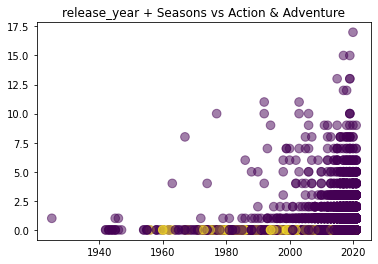
\includegraphics[width=0.3\textwidth]{Scatterplots/release+seasonvsaction.png}}
  \subfloat{
    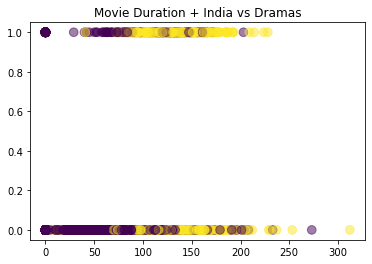
\includegraphics[width=0.3\textwidth]{Scatterplots/moviduration+indiavsromantic.png}}
  \subfloat{
    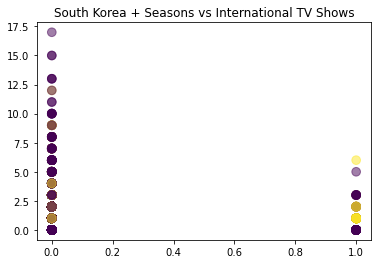
\includegraphics[width=0.3\textwidth]{Scatterplots/southkorea+seasonsvsinternational.png}}
  \label{fig:colores}
\end{figure}
\begin{figure}[h]
    \centering
    \subfloat{
    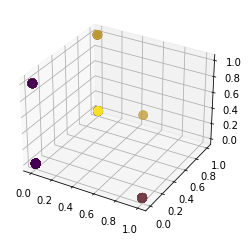
\includegraphics[width=0.3\textwidth]{Scatterplots/argentina+colombia+mexicovsspanish.png}}
  \subfloat{
    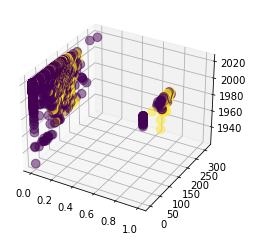
\includegraphics[width=0.3\textwidth]{Scatterplots/china+moviduration+releasevsaction.png}}
  \subfloat{
    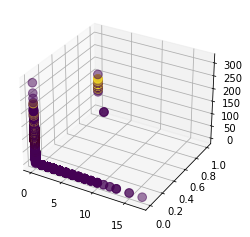
\includegraphics[width=0.3\textwidth]{Scatterplots/seasons+philipins+movidurationvsromantic.png}}
    \caption{Mostra dels \textit{scatterplots} en $\mathbb{R}^2$ i $\mathbb{R}^3$ generats per l'analisis exahustiu}
  \label{fig:colores}
\end{figure}\\
A partir de les imatges\footnote{La resta d'imatges es podenc onsultar al notebook entregat conjuntament amb la memória} generades\footnote{A la imatge es representa la variable objectiu com el color (lila o groc, no pertany o pertany respectivament) i els atributs utilitzats com a eixos} es pot deduïr la no existencia de relacions dels atributs amb la variable objectiu.\\
\begin{figure}[h] % Flotante "comun", sin caption, en que irán ambos
\begin{minipage}{7.5cm} % Minipagina para la tabla. 8 cm de ancho
\begin{center}
    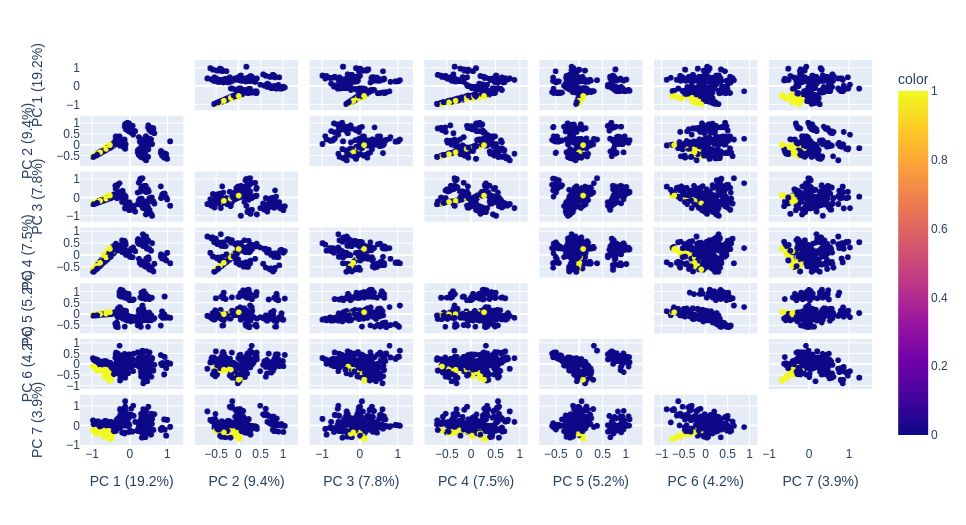
\includegraphics[width = 1 \textwidth]{PCA.png}
    \caption{PCA de la variable objectiu \textit{Comedies TV} amb els seus atributs més rellevants}
    \label{fig:my_label}
\end{center}
\end{minipage} % Fin de la minipagina de la tabla
\hspace{2em}
%\hfill % Espacio flexible para separar tabla y figura
\begin{minipage}{6cm} % Minipágina para la figura, 6 cm de ancho
Per tal de poder obtenir un millor enteniment de les distribucions de les daes i les relacions entre elles i la variable objectiu, és procedeix a fer una PCA de les variables objectius respecte als atributs més rellevants que hi corresponen.\\
En les imatges obtingudes com la PCA no obté resultats resenyables o minimament decents per a obtenir una bona classificació.\\
És procedeix a estudiar les interacions de diversos classificadors amb les variables objectius.
\end{minipage} % Fin de la minipagina que lleva la foto
\end{figure}





\newpage
\section{Classificació del dataset}\label{classificacio}
\subsection{Logistic Regressor} \label{logistic}
\subsubsection{Estudi de la precisió}
S'inicia l'estudi observant la precisió del model logístic amb paràmetres estàndard.\\
El resultat d'aplicar un regressor logístic (per a cadascuna de les variables objectius) per a classificar el dataset (sense utilitzar part del mateix per a validar) és:
\begin{figure}[h] % Flotante "comun", sin caption, en que irán ambos
\begin{minipage}{5cm} % Minipagina para la tabla. 8 cm de ancho
\begin{center}
    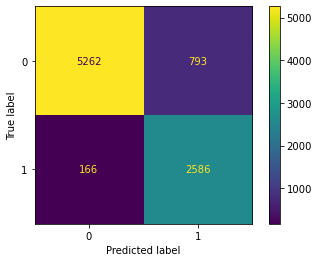
\includegraphics[width=1\textwidth]{ConfMatrix/CM_log_internationalMovie.png}
    \caption{\textit{Confusion matrix} del model logístic estàndard per \textit{International Movie}}
    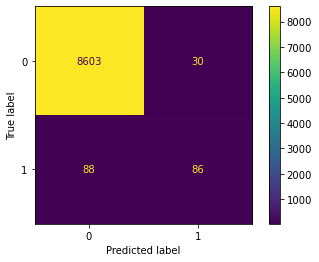
\includegraphics[width=1\textwidth]{ConfMatrix/CM_log_Spanish.png}
    \caption{\textit{Confusion matrix} del model logístic estàndard per \textit{Spanish-Language TV Shows}}
\end{center}
\end{minipage} % Fin de la minipagina de la tabla
\hspace{2em}
%\hfill % Espacio flexible para separar tabla y figura
\begin{minipage}{9cm} % Minipágina para la figura, 6 cm de ancho
\begin{center}
    \begin{tabular}{l|l|l}
        \textbf{Gènere} & \textbf{Atribut} & \textbf{Precissió}\\\hline\hline
            \multirow{3}{*}{International TV} &  Taiwan & \multirow{3}{*}{0.945} \\
            & United States & \\
            & Movie Duration& \\ \hline
        \multirow{2}{*}{Dramas} &  Movie Duration & \multirow{2}{*}{0.447} \\
        & India & \\ \hline
        \multirow{3}{*}{International Movie} &  India & \multirow{3}{*}{0.945} \\
            & United States & \\
            & Seasons & \\ \hline
        \multirow{3}{*}{British TV} &  United Kingdom & \multirow{3}{*}{0.889} \\
            & Movie Duration & \\
            & Seasons & \\ \hline
        \multirow{3}{*}{Spanish-Language} &  Spain & \multirow{3}{*}{0.494} \\
            & Movie Duration & \\
            & Mexico & \\ \hline
        \multirow{2}{*}{Anime Series} &  Movie Duration & \multirow{2}{*}{0.813} \\
        & Japan & \\\hline
        \multirow{2}{*}{Korean TV} &  Movie Duration & \multirow{2}{*}{0.874} \\
        & South Korea & \\
    \end{tabular}
    \label{tab:afins}
    \\
    Taula 4: Mostra de la recall de les variables objectius mitjançant un classificador logístic estandard   \setcounter{table}{4}
\end{center}
Es representen en una taula els resultats obtinguts pel classificador Logístic per aquelles variables objectius que no obté una precissió superior al $30\%$.
\end{minipage} % Fin de la minipagina que lleva la foto
\end{figure} % Fin del entorno comun. No lleva caption
\\
És conclou que el classificador logístic té, inicialment, bona capacitat de classificació. Pel que és recurreix a fer un cross validation per tal de corrovorar els resultats obtinguts.\\\\
Mencionar que les matrius de confució mostrades són un exemple de les obtingudes en la cerca del millors atributs per a classificar la variable objectiu mencionada com a peu d'imatge.\\
\newpage
\subsubsection{Cross Validation}
Al aplicar un \textit{cross validation} (amb 10 subdivisions del dataset) s'obté les següents precissions (mostrem només les que tenen una precissió major a $30\%$):
\begin{table}[h]
    \centering
    \begin{tabular}{l|l|l}
        \textbf{Gènere} & \textbf{Atribut} & \textbf{Precissió}\\\hline\hline
            \multirow{2}{*}{International TV} & United States & \multirow{2}{*}{0.945}\\
            & Movie Duration& \\ \hline
        \multirow{2}{*}{Dramas} &  Movie Duration & \multirow{2}{*}{0.447} \\
        & India & \\ \hline
        \multirow{3}{*}{International Movie} & United States & \multirow{3}{*}{0.94} \\
            & Seasons & \\ \hline
        \multirow{2}{*}{British TV} &  United Kingdom & \multirow{2}{*}{0.889} \\
            & Movie Duration & \\\hline
        \multirow{3}{*}{Spanish-Language} &  Spain & \multirow{3}{*}{0.492} \\
            & Movie Duration & \\
            & Mexico & \\ \hline
        \multirow{2}{*}{Anime Series} &  Movie Duration & \multirow{2}{*}{0.813} \\
        & Japan & \\\hline
        \multirow{2}{*}{Korean TV} &  Movie Duration & \multirow{2}{*}{0.874} \\
        & South Korea & \\
    \end{tabular}
    \caption{Mostra de la recall de les variables objectius mitjançant un CrossValidation}
    \label{tab:my_label}
\end{table}\\
És conclou que el classificador logístic permet de manera molt eficient classificar algunes variables objectiu; ja que tot i aplicar un CrossValidation amb 10 Kfolds obté molt bona recall i no cambia gairé be res respecte a la recall obtinguda amb totes les dades, no ésta tenint overfitting.\\\\
És prosegueix l'analisis dels classificadors provant altres models per millorar les prediccions del model logístic o obtenir més resultats eficients que el model logístic.
\newpage


\subsection{K-Nearest Neighbors}\label{KNN}
\subsubsection{Estudi de la precisió}
Es continua l'estudi observant la precisió del model KNN amb paràmetres estàndards, ja que al tractar-se d'un dataset amb dades molt compactes podria obtenir bons resultats.\\
El resultat d'aplicar aquest model (per a cadascuna de les variables objectius) per a classificar el dataset (sense utilitzar part del mateix per a validar) és:
\begin{figure}[h] % Flotante "comun", sin caption, en que irán ambos
\begin{minipage}{5cm} % Minipagina para la tabla. 8 cm de ancho
\begin{center}
    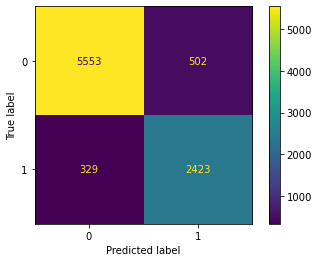
\includegraphics[width=1\textwidth]{ConfMatrix/CM_knn_intenationalmovie.png}
    \caption{\textit{Confusion matrix} del model K-Nearest Neighbour estàndard (K = 5) per \textit{International Movie}}
    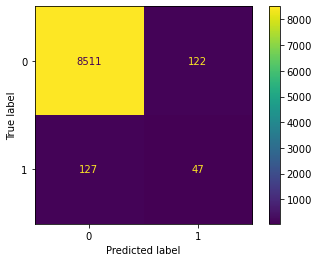
\includegraphics[width=1\textwidth]{ConfMatrix/CM_knn_spanish.png}
    \caption{\textit{Confusion matrix} del model K-Nearest Neighbour estàndard (K = 5)per \textit{Spanish-Language TV Shows}}
\end{center}
\end{minipage} % Fin de la minipagina de la tabla
\hspace{2em}
%\hfill % Espacio flexible para separar tabla y figura
\begin{minipage}{9cm} % Minipágina para la figura, 6 cm de ancho
\begin{center}
    \begin{tabular}{l|l|l}
        \textbf{Gènere} & \textbf{Atribut} & \textbf{Precissió}\\\hline\hline
            \multirow{2}{*}{TV Dramas} &  Seasons & \multirow{2}{*}{0.7} \\
            & Movie Duration& \\ \hline
        \multirow{3}{*}{Romantic TV} &  Seasons & \multirow{3}{*}{0.33} \\
        & South Korea & \\
            & Taiwan & \\ \hline
        \multirow{3}{*}{TV Comedies} &  Seasons & \multirow{3}{*}{0.349} \\
        & Movie Duration & \\
        & Taiwan & \\ \hline
        \multirow{3}{*}{Dramas} &  Movie Duration & \multirow{3}{*}{0.548} \\
        & India & \\ 
        & Seasons & \\\hline
        \multirow{3}{*}{International Movie} &  India & \multirow{3}{*}{0.945} \\
            & United States & \\
            & Seasons & \\ \hline
        \multirow{3}{*}{British TV} &  United Kingdom & \multirow{3}{*}{0.889} \\
            & Movie Duration & \\
            & Seasons & \\ \hline
        \multirow{3}{*}{Spanish-Language} &  Spain & \multirow{3}{*}{0.632} \\
            & Colombia & \\
            & Mexico & \\ \hline
        Classic Movies & Released Year & 0.491 \\
    \end{tabular}
    \label{tab:afins}
    \\
    Taula 7: Mostra de la recall de les variables objectius mitjançant un classificador KNN estandard   \setcounter{table}{7}
\end{center}
Es representen en una taula els resultats obtinguts pel classificador KNN per aquelles variables objectius que no obté una precissió superior al $30\%$.
\end{minipage} % Fin de la minipagina que lleva la foto
\end{figure} % Fin del entorno comun. No lleva caption
\\
És conclou que el classcadorifi KNN té, inicialment, bona capacitat de classificació. Pel que és recurreix a fer un cross validation per tal de corrovorar els resultats obtinguts.\\\\
A més, s'observa com té variables objectius que classifica de manera decent diferents a les obtingudes amb el regressor logístic, pel que és disposa a cambiar la dinàmica (de fer un model diferents per variable objectiu) a fer un classificador diferents per cada model (segons classifiqui millor).\\\\
Mencionar que les matrius de confució mostrades, al igual que en el regressor logístic, són un exemple de les obtingudes en la cerca del millors atributs per a classificar la variable objectiu mencionada com a peu d'imatge.\\
En futures explicacions de models son mostrades també exemples trobats.
\newpage 

\subsubsection{Cross Validation}
Al aplicar un \textit{cross validation} (amb 10 subdivisions del dataset) s'obté les següents precissions (mostrem només les que tenen una precissió major a $30\%$):
\begin{table}[h]
    \centering
    \begin{tabular}{l|l|l}
        \textbf{Gènere} & \textbf{Atribut} & \textbf{Precissió}\\\hline\hline
            \multirow{3}{*}{International TV} &  United States & \multirow{3}{*}{0.945} \\
            & India & \\
            & Movie Duration& \\ \hline
        \multirow{2}{*}{Dramas} &  Movie Duration & \multirow{2}{*}{0.5} \\ 
        & Seasons & \\\hline
        \multirow{2}{*}{International Movie} &  United States & \multirow{2}{*}{0.94} \\
            & Seasons & \\ \hline
        \multirow{2}{*}{British TV} &  United Kingdom & \multirow{2}{*}{0.889} \\
            & Movie Duration &  \\ \hline
        \multirow{3}{*}{Spanish-Language} &  Spain & \multirow{3}{*}{0.487} \\
            & Movie Duration & \\
            & Mexico & \\ \hline
        Classic Movies & Released Year & 0.38 \\ \hline
        \multirow{2}{*}{Anime Series} & Movie Duration & \multirow{2}{*}{0.813}\\
        & Japan & \\ \hline
        \multirow{2}{*}{Korean TV} & Movie Duration & \multirow{2}{*}{0.874}\\
        & South Korea & \\ 
        
    \end{tabular}
    \caption{Mostra de la recall de les variables objectius mitjançant un CrossValidation}
    \label{tab:my_label}
\end{table}\\
És conclou que el classificador KNN permet de manera molt eficient classificar algunes variables objectiu; ja que tot i aplicar un CrossValidation amb 10 Kfolds obté molt bona recall.\\\\
Tot i així, s'observa com cambia la recall respecte obtinguda amb totes les dades en algunes variables de manera significativa, pel que pot estar tenint overfitting; és tindrà cura aquesta circunstacia en futurs estudis més exahustius del mètode.\\\\

\newpage



\subsection{Support Vector Classification}\label{SVC}
\subsubsection{Estudi de la precisió}
Es continua l'estudi observant la precisió del model SVC amb paràmetres estàndards, ja que al tractar-se d'un dataset que ha funcionat de manera decent amb un classificador logístic podria obtenir bons resultats.\\
El resultat d'aplicar aquest model (per a cadascuna de les variables objectius) per a classificar el dataset (sense utilitzar part del mateix per a validar) és:
\begin{figure}[h] % Flotante "comun", sin caption, en que irán ambos
\begin{minipage}{5cm} % Minipagina para la tabla. 8 cm de ancho
\begin{center}
    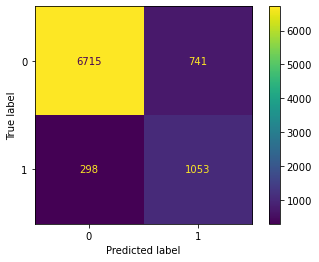
\includegraphics[width=1\textwidth]{ConfMatrix/CM_SVC_internationalTV.png}
    \caption{\textit{Confusion matrix} del model SVC per \textit{International TV Show}}
    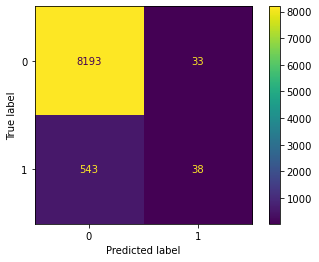
\includegraphics[width=1\textwidth]{ConfMatrix/CM_SVC_ComediesTV.png}
    \caption{\textit{Confusion matrix} del model SVC per \textit{Comedies TV Shows}}
\end{center}
\end{minipage} % Fin de la minipagina de la tabla
\hspace{2em}
%\hfill % Espacio flexible para separar tabla y figura
\begin{minipage}{9cm} % Minipágina para la figura, 6 cm de ancho
\begin{center}
    \begin{tabular}{l|l|l}
        \textbf{Gènere} & \textbf{Atribut} & \textbf{Precissió}\\\hline\hline
            \multirow{3}{*}{International TV} &  Taiwan & \multirow{3}{*}{0.945} \\
            & United States & \\
            & Movie Duration& \\ \hline
        \multirow{2}{*}{Dramas} &  Movie Duration & \multirow{2}{*}{0.437} \\
        & Seasons & \\\hline
        \multirow{3}{*}{International Movie} &  India & \multirow{3}{*}{0.94} \\
            & United States & \\
            & Seasons & \\ \hline
        \multirow{3}{*}{British TV} &  United Kingdom & \multirow{3}{*}{0.889} \\
            & Movie Duration & \\
            & Seasons & \\ \hline
        \multirow{3}{*}{Spanish-Language} &  Spain & \multirow{3}{*}{0.483} \\
            & Movie Duration & \\
            & Mexico & \\ \hline
        Classic Movies & Released Year & 0.397 \\ \hline 
        \multirow{2}{*}{Anime Series} & Movie Duration & \multirow{2}{*}{0,813}\\
        & Japan & \\ \hline
        \multirow{2}{*}{Korean TV} & Movie Duration & \multirow{2}{*}{0,874}\\
        & South Korea & \\ 
        
    \end{tabular}
    \label{tab:afins}
    \\
    Taula 11: Mostra de la recall de les variables objectius mitjançant un classificador SVC estandard   \setcounter{table}{11}
\end{center}
Es representen en una taula els resultats obtinguts pel classificador SVC per aquelles variables objectius que no obté una precissió superior al $30\%$.
\end{minipage} % Fin de la minipagina que lleva la foto
\end{figure} % Fin del entorno comun. No lleva caption
\\
És conclou que el classificador SVC té, inicialment, bona capacitat de classificació. Pel que és recurreix a fer un cross validation per tal de corrovorar els resultats obtinguts.\\\\
Cal descatar com s'intueix (mitjançant totes les dades per ara analitzades) que hi existeix una tendencia, tant en la recall com en els atributs) en els models a l'hora de classificar els gèneres. Aquesta tendencia a tenir valors semblant indica que, efectivament, les variables que s'estàn utilitzant són les que millor hi representen la classe; tot i que també reflexa un cert límit que podem assolïr amb elles i, a menys que en futurs classificadors utilitcin altres o classifiquin de millor manera que fins els ara vist, per tant pot haber variables objectius que siguin incapaces de ser classificades de forma decent per la  falta de dades o d'informació.
\newpage 

\subsubsection{Cross Validation}
Al aplicar un \textit{cross validation} (amb 10 subdivisions del dataset) s'obté les següents precissions (mostrem només les que tenen una precissió major a $30\%$):
\begin{table}[h]
    \centering
    \begin{tabular}{l|l|l}
        \textbf{Gènere} & \textbf{Atribut} & \textbf{Precissió}\\\hline\hline
            \multirow{2}{*}{International TV} &  United States & \multirow{2}{*}{0.945} \\
            & Movie Duration& \\ \hline
        \multirow{2}{*}{Dramas} &  Movie Duration & \multirow{2}{*}{0.443} \\ 
        & Seasons & \\\hline
        \multirow{2}{*}{International Movie} &  United States & \multirow{2}{*}{0.94} \\
            & Seasons & \\ \hline
        \multirow{2}{*}{British TV} &  United Kingdom & \multirow{2}{*}{0.889} \\
            & Movie Duration &  \\ \hline
        \multirow{3}{*}{Spanish-Language} &  Spain & \multirow{3}{*}{0.481} \\
            & Movie Duration & \\
            & Mexico & \\ \hline
        Classic Movies & Released Year & 0.381 \\ \hline
        \multirow{2}{*}{Anime Series} & Movie Duration & \multirow{2}{*}{0.813}\\
        & Japan & \\ \hline
        \multirow{2}{*}{Korean TV} & Movie Duration & \multirow{2}{*}{0.874}\\
        & South Korea & \\ 
        
    \end{tabular}
    \caption{Mostra de la recall de les variables objectius mitjançant un CrossValidation}
    \label{tab:my_label}
\end{table}\\
És conclou que el classificador SVC permet de manera molt eficient classificar algunes variables objectiu; ja que tot i aplicar un CrossValidation amb 10 Kfolds obté molt bona recall.\\\\
Cal esmentar com, es pot conjeturar l'hipotesis abans proposada que hi existeix un cert límit que hi podem arribar a obtenir com a recall per als atributs mitjançant les dades que hi disposem. \\
Per tal d'intentar evitar aquest cas i superar aquest hipotétic umbral, és procedeix a probar models de classificació basants en altres tecniques de classificació.

\newpage


\subsection{Decision Tree Classificator}\label{TREE}
\subsubsection{Estudi de la precisió}
Es continua l'estudi observant la precisió del model Decission Tree Classifier amb paràmetres estàndards, ja que al tractar-se d'un dataset que ha funcionat de manera decent amb un classificador logístic podria obtenir bons resultats.\\
El resultat d'aplicar aquest model (per a cadascuna de les variables objectius) per a classificar el dataset (sense utilitzar part del mateix per a validar) és:
\begin{figure}[h] % Flotante "comun", sin caption, en que irán ambos
\begin{minipage}{5cm} % Minipagina para la tabla. 8 cm de ancho
\begin{center}
    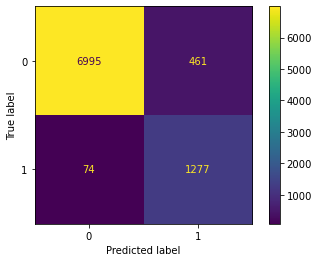
\includegraphics[width=1\textwidth]{ConfMatrix/CM_DT_InternationalTV.png}
    \caption{\textit{Confusion matrix} del model Decission Tree per \textit{International TV Show}}
    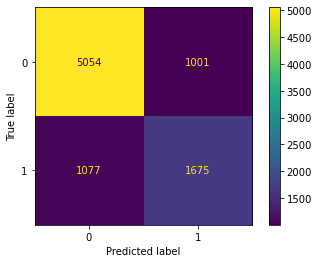
\includegraphics[width=1\textwidth]{ConfMatrix/CM_DT_InternationalMovies.png}
    \caption{\textit{Confusion matrix} del model Decission Tree per \textit{International Movies}}
\end{center}
\end{minipage} % Fin de la minipagina de la tabla
\hspace{2em}
%\hfill % Espacio flexible para separar tabla y figura
\begin{minipage}{9cm} % Minipágina para la figura, 6 cm de ancho
\begin{center}
    \begin{tabular}{l|l|l}
        \textbf{Gènere} & \textbf{Atribut} & \textbf{Precissió}\\\hline\hline
            \multirow{3}{*}{International TV} &  Taiwan & \multirow{3}{*}{0.945} \\
            & United States & \\
            & Movie Duration& \\ \hline
        \multirow{3}{*}{Romantic TV} &  Taiwan & \multirow{3}{*}{0.332} \\
            & South Korea & \\
            & Seasons & \\ \hline
        \multirow{2}{*}{Dramas} &  Movie Duration & \multirow{2}{*}{0.55} \\
        & Seasons & \\\hline
        \multirow{3}{*}{International Movie} &  India & \multirow{3}{*}{0.94} \\
            & United States & \\
            & Seasons & \\ \hline
        \multirow{3}{*}{British TV} &  United Kingdom & \multirow{3}{*}{0.889} \\
            & Movie Duration & \\
            & Seasons & \\ \hline
        \multirow{3}{*}{Spanish-Language} &  Spain & \multirow{3}{*}{0.494} \\
            & Movie Duration & \\
            & Mexico & \\ \hline
        Classic Movies & Released Year & 0.457 \\ \hline 
        \multirow{2}{*}{Anime Series} & Movie Duration & \multirow{2}{*}{0.813}\\
        & Japan & \\ \hline
        \multirow{2}{*}{Korean TV} & Movie Duration & \multirow{2}{*}{0.874}\\
        & South Korea & \\ 
        
    \end{tabular}
    \label{tab:afins}
    \\
    Taula 11: Mostra de la recall de les variables objectius mitjançant un classificador Decission Tree estandard   \setcounter{table}{11}
\end{center}
Es representen en una taula els resultats obtinguts pel classificador Decission Tree per aquelles variables objectius que no obté una precissió superior al $30\%$.
\end{minipage} % Fin de la minipagina que lleva la foto
\end{figure} % Fin del entorno comun. No lleva caption
\\
És conclou que el classificador Decission Tree té, inicialment, bona capacitat de classificació. Pel que és recurreix a fer un cross validation per tal de corrovorar els resultats obtinguts.\\\\

\newpage 

\subsubsection{Cross Validation}
Al aplicar un \textit{cross validation} (amb 10 subdivisions del dataset) s'obté les següents precissions (mostrem només les que tenen una precissió major a $30\%$):
\begin{table}[h]
    \centering
    \begin{tabular}{l|l|l}
        \textbf{Gènere} & \textbf{Atribut} & \textbf{Precissió}\\\hline\hline
            \multirow{2}{*}{International TV} &  United States & \multirow{2}{*}{0.945} \\
            & Movie Duration& \\ \hline
        \multirow{2}{*}{Dramas} &  Movie Duration & \multirow{2}{*}{0.498} \\ 
        & Seasons & \\\hline
        \multirow{2}{*}{International Movie} &  United States & \multirow{2}{*}{0.94} \\
            & Seasons & \\ \hline
        \multirow{2}{*}{British TV} &  United Kingdom & \multirow{2}{*}{0.889} \\
            & Movie Duration &  \\ \hline
        \multirow{3}{*}{Spanish-Language} &  Spain & \multirow{3}{*}{0.487} \\
            & Movie Duration & \\
            & Mexico & \\ \hline
        Classic Movies & Released Year & 0.38 \\ \hline
        \multirow{2}{*}{Anime Series} & Movie Duration & \multirow{2}{*}{0.813}\\
        & Japan & \\ \hline
        \multirow{2}{*}{Korean TV} & Movie Duration & \multirow{2}{*}{0.874}\\
        & South Korea & \\ 
        
    \end{tabular}
    \caption{Mostra de la recall de les variables objectius mitjançant un CrossValidation}
    \label{tab:my_label}
\end{table}\\
És conclou que el classificador Decission Tree permet de manera molt eficient classificar algunes variables objectiu; ja que tot i aplicar un CrossValidation amb 10 Kfolds obté molt bona recall.\\\\
També mencionar que no ha pogut predir de manera més eficient que la resta de classificadors probats fins ara els atributs que menys recall obtenen, pel que és probarà mitjançant un ensemble de Decission Trees dur a terme aquesta tasca.
\newpage


\subsection{Random Forest Classificator}\label{random}
\subsubsection{Estudi de la precisió}
Es continua l'estudi observant la precisió del model Random Forest Classifier amb paràmetres estàndards, ja que al tractar-se d'un dataset que ha funcionat de manera decent amb un classificador Decission Tree, podria obtenir bons resultats.\\
El resultat d'aplicar aquest model (per a cadascuna de les variables objectius) per a classificar el dataset (sense utilitzar part del mateix per a validar) és:
\begin{figure}[h] % Flotante "comun", sin caption, en que irán ambos
\begin{minipage}{5cm} % Minipagina para la tabla. 8 cm de ancho
\begin{center}
    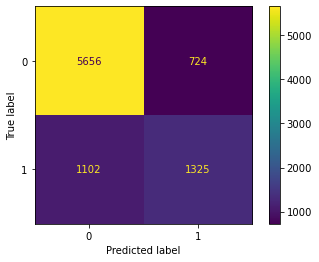
\includegraphics[width=1\textwidth]{ConfMatrix/CM_RF_Dramas.png}
    \caption{\textit{Confusion matrix} del model Random Forest per \textit{Dramas}}
    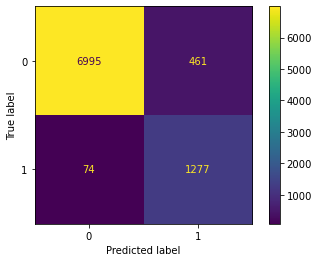
\includegraphics[width=1\textwidth]{ConfMatrix/CM_RF_InternationalTV.png}
    \caption{\textit{Confusion matrix} del model Random Forest per \textit{International TV Show}}
\end{center}
\end{minipage} % Fin de la minipagina de la tabla
\hspace{2em}
%\hfill % Espacio flexible para separar tabla y figura
\begin{minipage}{9cm} % Minipágina para la figura, 6 cm de ancho
\begin{center}
    \begin{tabular}{l|l|l}
        \textbf{Gènere} & \textbf{Atribut} & \textbf{Precissió}\\\hline\hline
            \multirow{3}{*}{International TV} &  Taiwan & \multirow{3}{*}{0.945} \\
            & United States & \\
            & Movie Duration& \\ \hline
        \multirow{3}{*}{Romantic TV} &  Taiwan & \multirow{3}{*}{0.332} \\
            & South Korea & \\
            & Seasons & \\ \hline
        \multirow{2}{*}{Dramas} &  Movie Duration & \multirow{2}{*}{0.592} \\
        & Seasons & \\\hline
        \multirow{3}{*}{International Movie} &  India & \multirow{3}{*}{0.94} \\
            & United States & \\
            & Seasons & \\ \hline
        \multirow{3}{*}{British TV} &  United Kingdom & \multirow{3}{*}{0.889} \\
            & Movie Duration & \\
            & Seasons & \\ \hline
        \multirow{3}{*}{Spanish-Language} &  Spain & \multirow{3}{*}{0.494} \\
            & Movie Duration & \\
            & Mexico & \\ \hline
        Classic Movies & Released Year & 0.422 \\ \hline 
        \multirow{2}{*}{Anime Series} & Movie Duration & \multirow{2}{*}{0.813}\\
        & Japan & \\ \hline
        \multirow{2}{*}{Korean TV} & Movie Duration & \multirow{2}{*}{0.874}\\
        & South Korea & \\ 
        
    \end{tabular}
    \label{tab:afins}
    \\
    Taula 13: Mostra de la recall de les variables objectius mitjançant un classificador Random Forest estandard   \setcounter{table}{13}
\end{center}
Es representen en una taula els resultats obtinguts pel classificador Decission Tree per aquelles variables objectius que no obté una precissió superior al $30\%$.
\end{minipage} % Fin de la minipagina que lleva la foto
\end{figure} % Fin del entorno comun. No lleva caption
\\
És conclou que el regressor Random Forest té, inicialment, bona capacitat de classificació. Pel que és recurreix a fer un cross validation per tal de corrovorar els resultats obtinguts.\\\\

\newpage 

\subsubsection{Cross Validation}
Al aplicar un \textit{cross validation} (amb 10 subdivisions del dataset) s'obté les següents precissions (mostrem només les que tenen una precissió major a $30\%$):
\begin{table}[h]
    \centering
    \begin{tabular}{l|l|l}
        \textbf{Gènere} & \textbf{Atribut} & \textbf{Precissió}\\\hline\hline
            \multirow{2}{*}{International TV} &  United States & \multirow{2}{*}{0.945} \\
            & Movie Duration& \\ \hline
        \multirow{2}{*}{Dramas} &  Movie Duration & \multirow{2}{*}{0.503} \\ 
        & Seasons & \\\hline
        \multirow{2}{*}{International Movie} &  United States & \multirow{2}{*}{0.94} \\
            & Seasons & \\ \hline
        \multirow{2}{*}{British TV} &  United Kingdom & \multirow{2}{*}{0.889} \\
            & Movie Duration &  \\ \hline
        \multirow{3}{*}{Spanish-Language} &  Spain & \multirow{3}{*}{0.487} \\
            & Movie Duration & \\
            & Mexico & \\ \hline
        Classic Movies & Released Year & 0.414 \\ \hline
        \multirow{2}{*}{Anime Series} & Movie Duration & \multirow{2}{*}{0.813}\\
        & Japan & \\ \hline
        \multirow{2}{*}{Korean TV} & Movie Duration & \multirow{2}{*}{0.874}\\
        & South Korea & \\ 
        
    \end{tabular}
    \caption{Mostra de la recall de les variables objectius mitjançant un CrossValidation}
    \label{tab:my_label}
\end{table}\\
És conclou que el classificador Random Forest permet de manera molt eficient classificar algunes variables objectiu; ja que tot i aplicar un CrossValidation amb 10 Kfolds obté molt bona recall.\\\\
També mencionar que no ha pogut dur a terme la tasca de obtenir bones prediccinos per a altres atributs als plasmats a les taules durant l'analisis dels models vist fins ara, pel que es recorrirà a altres mètodes de classificació.

\newpage

\subsection{Kmeans}\label{random}
\subsubsection{Estudi de la precisió}
Es continua l'estudi observant la precisió del model K-means Classifier amb paràmetres estàndards.\\
El resultat d'aplicar aquest model (per a cadascuna de les variables objectius) per a classificar el dataset (sense utilitzar part del mateix per a validar) és:
\begin{figure}[h] % Flotante "comun", sin caption, en que irán ambos
\begin{minipage}{5cm} % Minipagina para la tabla. 8 cm de ancho
\begin{center}
    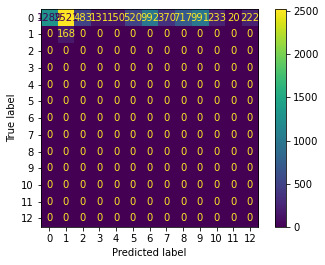
\includegraphics[width=1\textwidth]{ConfMatrix/CM_KM_Action.png}
    \caption{\textit{Confusion matrix} del model K-means per \textit{Action \& Adventures}}
    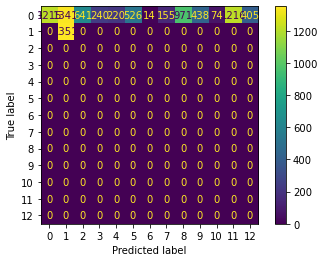
\includegraphics[width=1\textwidth]{ConfMatrix/CM_KM_InternationalTV.png}
    \caption{\textit{Confusion matrix} del model K-means per \textit{International TV Show}}
\end{center}
\end{minipage} % Fin de la minipagina de la tabla
\hspace{2em}
%\hfill % Espacio flexible para separar tabla y figura
\begin{minipage}{9cm} % Minipágina para la figura, 6 cm de ancho
\begin{center}
    \begin{tabular}{l|l|l}
        \textbf{Gènere} & \textbf{Atribut} & \textbf{Precissió}\\\hline\hline
            Documentaries & Seasons & 1.00 \\ \hline
        \multirow{2}{*}{Dramas} &  India & \multirow{2}{*}{0.727} \\
        & Seasons & \\\hline
        \multirow{3}{*}{International Movie} &  Seasons & \multirow{3}{*}{0.94} \\
            & United States & \\ \hline
        \multirow{3}{*}{Action \& Adventure} &  China 
 & \multirow{3}{*}{0.888} \\
            & Hong Kong & \\
            & Seasons & \\ \hline
        Anime Series & Japan & 0.859\\ 
    \end{tabular}
    \label{tab:afins}
    \\
    Taula 15: Mostra de la recall de les variables objectius mitjançant un classificador K-means estandard   \setcounter{table}{15}
\end{center}
Es representen en una taula els resultats obtinguts pel classificador Decission Tree per aquelles variables objectius que no obté una precissió superior al $30\%$.\\\\
S'observa de forma evident que el model pateix d'un fort overfitting ja que només és capaç de classificar 13 classes (ja que és el paràmetre estandard del K-means).\\\\
A més, observant la matriu de confusió, és plasma de manera evident la poca capacitat de classificació eficient que té el model.
\end{minipage} % Fin de la minipagina que lleva la foto
\end{figure} % Fin del entorno comun. No lleva caption
\\
És conclou que el classificador K-means té, inicialment, bona capacitat de classificació peró no amb el paràmetre estandard.\\\\
No és procedirà amb el CrossValidation i, és retornarà a estudiar el cas més endabant en la cerca de hiperparàmetres per si consegueix així corretgir el comportament.\\\\
És procedeix doncs amb un altre model similar al K-means per a intentar obtenir resultats millors amb aquest sistema de classificació.

\newpage


\subsection{Gaussian Mixture}\label{random}
\subsubsection{Estudi de la precisió}
Es continua l'estudi observant la precisió del model Gaussian Mixture Classifier amb paràmetres estàndards.\\
El resultat d'aplicar aquest model (per a cadascuna de les variables objectius) per a classificar el dataset (sense utilitzar part del mateix per a validar) és:
\begin{figure}[h] % Flotante "comun", sin caption, en que irán ambos
\begin{minipage}{5cm} % Minipagina para la tabla. 8 cm de ancho
\begin{center}
    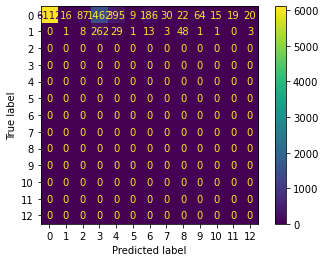
\includegraphics[width=1\textwidth]{ConfMatrix/CM_GM_RomanticTV.png}
    \caption{\textit{Confusion matrix} del model Gaussian Mixture per \textit{Romantic TV Show}}
    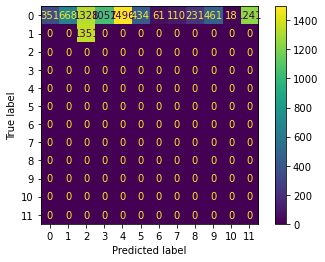
\includegraphics[width=1\textwidth]{ConfMatrix/CM_GM_InternationalTV.png}
    \caption{\textit{Confusion matrix} del model Gaussian Mixture per \textit{International TV Show}}
\end{center}
\end{minipage} % Fin de la minipagina de la tabla
\hspace{2em}
%\hfill % Espacio flexible para separar tabla y figura
\begin{minipage}{9cm} % Minipágina para la figura, 6 cm de ancho
\begin{center}
    \begin{tabular}{l|l|l}
        \textbf{Gènere} & \textbf{Atribut} & \textbf{Precissió}\\\hline\hline
        \multirow{2}{*}{International TV} &  Japan & \multirow{2}{*}{0.840} \\
        & United States & \\\hline
        \multirow{2}{*}{International Movie} &  India & \multirow{2}{*}{0.631} \\
            & United States & \\ \hline
        Anime Series & Japan & 0.859\\ 
    \end{tabular}
    \label{tab:afins}
    \\
    Taula 17: Mostra de la recall de les variables objectius mitjançant un classificador Gaussian Mixture estandard   \setcounter{table}{17}
\end{center}
Es representen en una taula els resultats obtinguts pel classificador Gaussian Mixture per aquelles variables objectius que no obté una precissió superior al $30\%$.\\\\
S'observa de forma evident que el model pateix d'un fort overfitting i d'incapacitat per a classificar de manera adient.\\\\
També es pot observar aquesta poca capacitat de classificació eficient que té el model mitjançant les matrius de confució.
\end{minipage} % Fin de la minipagina que lleva la foto
\end{figure} % Fin del entorno comun. No lleva caption
\\
És conclou que el classificador Gaussian Mixture té, inicialment, bona capacitat de classificació peró no amb el paràmetre estandard.\\\\
No és procedirà amb el CrossValidation i, és retornarà a estudiar el cas més endabant en la cerca de hiperparàmetres per si consegueix així corretgir el comportament.\\\\
És procedeix doncs a probar altres mètodes més sofisticats per classificar.
\newpage

\subsection{Models de xarxes neural}\label{random}
\subsubsection{Estudi de la precisió}
Es continua l'estudi observant la precisió de diversos models mitjançant xarxes neural deferents.\\
S'ha definit 4 models diferents que tenen com a diferencia unica el \textit{hidden layers}.\\
És mostre ara els resultats de cada model:
\begin{figure}[h] % Flotante "comun", sin caption, en que irán ambos
\begin{minipage}{7cm} % Minipagina para la tabla. 8 cm de ancho
\begin{center}
    \begin{tabular}{l|l|l}
        \textbf{Gènere} & \textbf{Model} & \textbf{Precissió}\\\hline\hline
        International TV & 4 & 0.926\\ \hline
        Dramas &  3 &  0.567 \\\hline
        International Movie &  3 & 0.913 \\ \hline
        British TV & 2 & 0.868 \\ \hline
        Anime Features & 3 & 0.809\\ \hline
        Anime Series & 3 & 0.887\\ \hline
        Korean TV & 3 & 0.689\\ \hline
        Stand-Up Comedy & 3 & 0.34 \\
    \end{tabular}
    \label{tab:afins}
    \\
    Taula 18: Mostra de la recall de les variables objectius mitjançant xarxes neurals  \setcounter{table}{18}
\end{center}
\end{minipage} % Fin de la minipagina de la tabla
\hspace{2em}
%\hfill % Espacio flexible para separar tabla y figura
\begin{minipage}{7cm} % Minipágina para la figura, 6 cm de ancho

Es representen en una taula els resultats obtinguts pels models de xarxes neurals proposats per aquelles variables objectius que obté una precissió superior al $30\%$.\\\\
S'observa que el model no té una bona precissió (o almenys en comparació a altres models ja analitzats); tot i així, obté bons resultats en atributs que no han estat classificats de forma adient fins ara.\\\\
Mencionar, que els models proposats han estat creats de forma intuïtiva i que, per tant, és pot refinar la seva estructura per a obtenir millors classificacions.
\end{minipage} % Fin de la minipagina que lleva la foto
\end{figure} % Fin del entorno comun. No lleva caption
\\
És conclou que la xarxa neural model 3 té, inicialment, bona capacitat de classificació per certs atributs fins ara no classificats de forma adient.\\\\
És procedirà a estudiar les xarxes neurals amb estructura similar a la del model 3 per tal de trobar altres atributs que puguin ser classificables amb aquests mètodes de classificació.\\
\begin{table}[h]
    \centering
    \begin{tabular}{c|c}
        \textbf{Model} & \textbf{Estructura/distribució en la \textit{hidden layer}} \\ \hline \hline
        Model 1 & 1 capa de 5 nodes\\ \hline
        Model 2 & 2 capes de 10 nodes cadascuna \\ \hline
        Model 3 & 2 capes de 20 nodes cadascuna \\ \hline
        Model 4 & 3 capes de 50 nodes cadascuna \\ 
    \end{tabular}
    \caption{Models proposats com a xarxes neurals de classificació}
    \label{tab:my_label}
\end{table}
\newpage
\subsection{Estudi del model de xarxa neural 3}
És procedeix a fer un estudi de la recall del model de xarxa neural 3 amb diferents valors de \textit{hidden layer}.\\
L'estructura de dues capes és manté peró és variarà el nombre de nodes de cadascuna amb valors que oscilin entre 15 i 31.
Els resultat d'aquest estudi son:

\begin{figure}[h] % Flotante "comun", sin caption, en que irán ambos
\begin{minipage}{7cm} % Minipagina para la tabla. 8 cm de ancho
\begin{center}
    \begin{tabular}{l|l|l}
        \textbf{Gènere} & \textbf{Nodes} & \textbf{Precissió}\\\hline\hline
        International TV & 20 & 0.936\\ \hline
        Romantic TV &  24 &  0.307 \\\hline
        Dramas &  23 &  0.582 \\\hline
        International Movie &  31 & 0.918 \\ \hline
        British TV & 22 & 0.868 \\ \hline
        Spanish-Language TV & 29 & 0.596 \\ \hline
        Anime Features & 20 & 0.809\\ \hline
        Anime Series & 16 & 0.886\\ \hline
        Korean TV & 24 & 0.889\\ \hline
        Stand-Up Comedy & 24 & 0.408 \\
    \end{tabular}
    \label{tab:afins}
    \\
    Taula 20: Mostra de la recall de les variables objectius mitjançant xarxes neurals de model 3 \setcounter{table}{20}
\end{center}
\end{minipage} % Fin de la minipagina de la tabla
\hspace{2em}
%\hfill % Espacio flexible para separar tabla y figura
\begin{minipage}{7cm} % Minipágina para la figura, 6 cm de ancho

Es representen en una taula els resultats obtinguts pels difersos models de tipus 3 de xarxa neural proposat anteriorment per aquelles variables objectius que obté una precissió superior al $30\%$.\\\\
S'observa clarament com el model obté precissions similars a les obtingudes per altres models més sencills plantejats anteriorment.\\\\
Per altra banda, també s'observa com el model amb 20 nodes és capaz de classificar de manera molt eficaç el gènere \textit{Anime Features} que fins ara no ha sigut classificat de manera eficient per cap classificador.
\end{minipage} % Fin de la minipagina que lleva la foto
\end{figure} % Fin del entorno comun. No lleva caption
\\
En l'estudi s'ha dividit el dataset en train i test per així evitar que el model memorítzi o pateixi d'overfitting.\\\\
Com que ha obtingut bons resultats el model, es proba a utilitzar els models abans testejats d'una manera més complexa per probar si, també, poden servir per a classificar altres gèneres.
\subsection{Estudi del model de xarxa neural 1}
Recuperant l'idea abans esmentada de crear un classificador que aprofiti les dades que ha obtingut altres classificador, s'aprofita els models de xarxes neurals descartats anteriorment per a testejar si tenen algun comportament que, amb les noves dades obtingudes mitjançant els classificadors que ja disposem, pot classificar altres gèneres.\\\\
El model que millor comportament ha tingut dels abans esmentats és el model de xarxa neural 1.\\\\
L'unic resultat resenyable és el de la variable objectiu \textit{TV Dramas} que obté amb el model 1 una recall de $0.593$\\\\
Tot i no haver-se obtingut millors ćlassificacions i més classificacions de variables objectiu, s'ha obtingut una certa millora al poder ara classificar mitjançant models de xarxes neurals 1 un gènere fins ara no classificat decentment mai.

\section{Plantejament del classificador}
Mitjançant totes les dades obtingudes, és conclou utilitzar el millor classificador per a cada variable i, a l'hora de classificar, ajuntar les classificacions fetes per cada classificador.\\\\
L'estudi del millor classificador obté els següents resultats:
\begin{table}[h]
    \centering
    \begin{tabular}{c|c|c|c}
        \textbf{Variable} & \textbf{Classificador} & \textbf{Atributs} & \textbf{Precissió}\\ \hline \hline
         International TV & Logístic & Movie Duration \& U.S.A. & 0.94 \\ \hline
         Dramas & Random Forest & Movie Duration \& Seasons & 0.56 \\ \hline 
         International Movies & Logístic & U.S.A. \& Seasons & 0.94 \\ \hline 
         British TV & Logístic & Movie Duration \& U.K. & 0.89 \\ \hline 
         Spanish-Lang. TV & Logístic & Spain \& Mexico \& Movie Duration & 0.51 \\ \hline 
         Anime Series & Logístic & Japan \& Movie Duration & 0.82 \\ \hline 
         Korean TV & Logístic & South Korea \& Movie Duration & 0.87\\\hline 
         Anime Features & Neural Network & \textit{ALL} & 0.81 \\ \hline \hline 
         TV Dramas & Neural Network & \textit{Classified types} & 0.59
    \end{tabular}
    \caption{Millor combinació d'atributs per al millor classificador de cada variable}
    \label{tab:my_label}
\end{table}\\
Mencionar que, en la taula, \textit{ALL} fa referencia a utilitzar tot els atributs i \textit{Classified types} fa referencia a les etiquetes proposades pels classificadors anterior a ella; per aquest motiu és separa la variable \textit{TV Dramas} de la resta, perque precissa de la classificació de les altres variables per classificar-la.\\\\
S'bserva com, tot i tenir poques correlacions rellevants per classificar, els classificadors de manera estandard són capaços d'obtenir una bona classificació en alguns atributs que, a més, són els que més dades tenen.\\
Per aquest motiu, és confirma la sospita que era casi impossible predir de forma eficient certes variables objectius per falta de dades.\\\\
És limitarà doncs a augmentar la precissió dels mètodes que hi disposem mitjançant una cerca d'hiperparàmetres per tal de trobar aquells que fan que la precissió sigui la més alta possible.\\\\
Per altra banda, surgeix l'idea de utilitzar el mateix concepte que amb la xarxa neural del model 1 amb la variable \textit{TV Dramas} per tal de classificar altres variables de la següent manera:
\begin{itemize}
    \item Utilitzar els classificador sencills per a predir els resultats més sencills.
    \item Utilitzar xarxes neurals especifiques per a etiquetar les variables més dificils de classificar.
    \item Utilitzar una xarxa neural que (iterada sobre ella mateixa K cops) rectifiqui els error d'etiquetatge i classifiqui millor les produccions.
\end{itemize}
\newpage 
Així doncs, l'idea de l'algorísme seria la següent:
\begin{enumerate}
    \item Classificar mitjançant els classificadors més sencills les variables més facils de classificar
    \item Afegir les classificacions a una llista d'etiquetes
    \item Mentres quedin variables sense etiquetar:
    \begin{enumerate}
        \item Classificar mitjançant una xarxa neural una variable no etiquetada amb totes les dades que s'hi disposen i la llista d'etiquetes obtingudes.
        \item afegir la classificació a la llista d'etiquetes
    \end{enumerate}
    \item Durant K-iteracions:
    \begin{enumerate}
        \item Utilitzar una xarxa neural que amb totes les classificacions fetes i totes les dades reclassifiqui les etiquetes. 
        \item Substituïr la llista d'etiquetes inicial per la obtinguda en la xarxa neural.
    \end{enumerate}
    \item Classificar la producció com la llista d'etiquetes obtinguda
\end{enumerate}
Aquesta idea d'algorisme no ha sigut testejada per falta de temps i no és pot assegurar que funcioni. \\\\
Tot i així, s'hagues intentat testejar aquest l'algorisme si s'hagues disposat de més temps. \\\\\\
És procedeix doncs, a estudiar les curves dels mètodes de classificació que hi disposem abans de fer la cerca d'hiperparàmetres per tal de, una vegada duta a terme la cerca, comparar-les.
\newpage
\section{Estudi de les curves Precission-Recall i ROC dels models}
\subsection{Precission-Recall i ROC curve dels models Logístics}
\begin{figure}[h]
\centering
    \subfloat[\textit{ROC curve}]{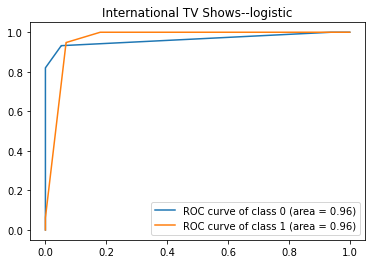
\includegraphics[width = 0.5 \textwidth]{ROCcurve/internationalTV_ROC.png}}
    \subfloat[\textit{Precission-Recall curve}]{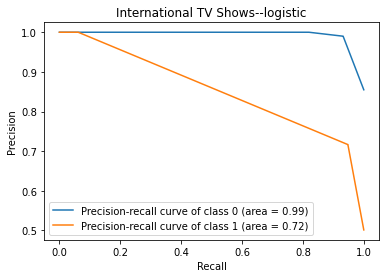
\includegraphics[width = 0.5 \textwidth]{PrecisionRecallCurve/InternationalTV_RECALL.png}}
    \caption{Corba \textit{ROC} i \textit{Precission-Recall} del model Logístic per la variable \textit{International TV Shows}}
    \label{fig:my_label}
\end{figure}
\hspace{-1.5em}S'observa de les curves ROC que el model te una bona sensibilitat, peró també s'observa de les curves Precission-Recall com hi existeix una tendencia a no tenir molt bona recall precissió i com la recall de les classes decau de forma lineal fins a un valor proper al $70\%$ en la classificació de la variable objectiu.\\\\
Tot i així te un bon resultat ja que les dues corves (ROC i Precission-Recall) obtenen valor propers a 1.
\begin{figure}[h]
\centering
    \subfloat[\textit{ROC curve}]{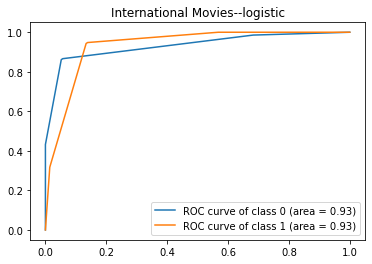
\includegraphics[width = 0.5 \textwidth]{ROCcurve/InternationalMovie_ROC.png}}
    \subfloat[\textit{Precission-Recall curve}]{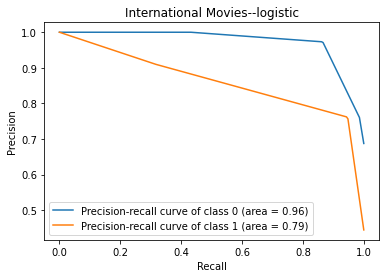
\includegraphics[width = 0.5 \textwidth]{PrecisionRecallCurve/InternationalMovies_RECALL.png}}
    \caption{Corba \textit{ROC} i \textit{Precission-Recall} del model Logístic per la variable \textit{International Movies}}
    \label{fig:my_label}
\end{figure}\\
S'observa de les corbes ROC i Precission-Recall un resultat similar al obtingut amb la variable \textit{International TV Show}.\\
Es conclou doncs que té un bon resultat ja que les dues corves (ROC i Precission-Recall) obtenen valors propers a 1.
\newpage
\begin{figure}[h]
\centering
    \subfloat[\textit{ROC curve}]{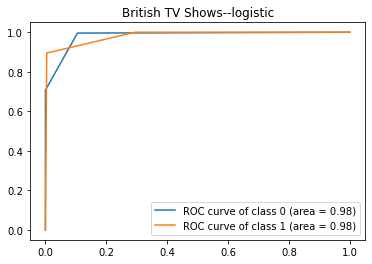
\includegraphics[width = 0.5 \textwidth]{ROCcurve/BritishTV_ROC.png}}
    \subfloat[\textit{Precission-Recall curve}]{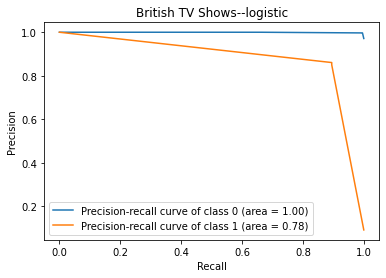
\includegraphics[width = 0.5 \textwidth]{PrecisionRecallCurve/BritishTV_RECALL.png}}
    \caption{Corba \textit{ROC} i \textit{Precission-Recall} del model Logístic per la variable \textit{British TV Shows}}
    \label{fig:my_label}
\end{figure}\\
\hspace{-1.5em}S'observa de les corbes ROC i Precission-Recall un resultat similar al obtingut amb la variable \textit{International TV Show}.\\
Es conclou doncs que té un bon resultat ja que les dues corves (ROC i Precission-Recall) obtenen valors propers a 1.
\begin{figure}[h]
\centering
    \subfloat[\textit{ROC curve}]{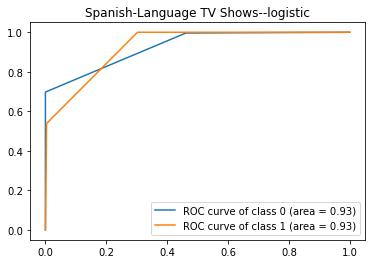
\includegraphics[width = 0.5 \textwidth]{ROCcurve/SpanishTV_ROC.png}}
    \subfloat[\textit{Precission-Recall curve}]{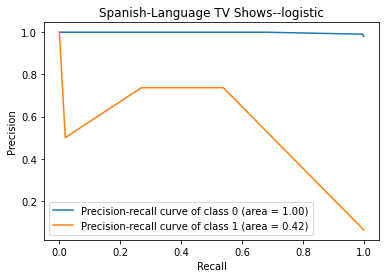
\includegraphics[width = 0.5 \textwidth]{PrecisionRecallCurve/SpanishTV_RECALL.png}}
    \caption{Corba \textit{ROC} i \textit{Precission-Recall} del model Logístic per la variable \textit{Spanish-Language TV Shows}}
    \label{fig:my_label}
\end{figure}\\
S'observa com el model de classificació logístic te problemes per distingir si una producció és o no de gènere \textit{Spanish-Language TV Show}; tot i així, dona bons resultats quan s'utilitza i és basntant eficient.\\\\
Es conclou doncs que té un resultat bo pero millorable i amb la cerca d'hiperparàmetres és milloraran aquests resultats.
\newpage 
\begin{figure}[h]
\centering
    \subfloat[\textit{ROC curve}]{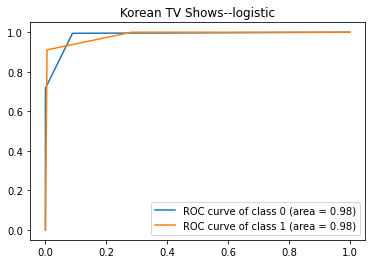
\includegraphics[width = 0.5 \textwidth]{ROCcurve/KoreanTV_ROC.png}}
    \subfloat[\textit{Precission-Recall curve}]{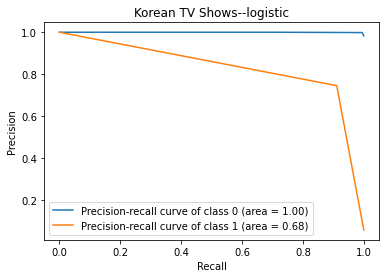
\includegraphics[width = 0.5 \textwidth]{PrecisionRecallCurve/KoreanTV_RECALL.png}}
    \caption{Corba \textit{ROC} i \textit{Precission-Recall} del model Logístic per la variable \textit{Korean TV Shows}}
    \label{fig:my_label}
\end{figure}\\
\hspace{-1.5em}S'observa de les corbes ROC i Precission-Recall un resultat similar al obtingut amb la variable \textit{International TV Show}.\\
Es conclou doncs que té un bon resultat ja que les dues corves (ROC i Precission-Recall) obtenen valors propers a 1.
\begin{figure}[h]
\centering
    \subfloat[\textit{ROC curve}]{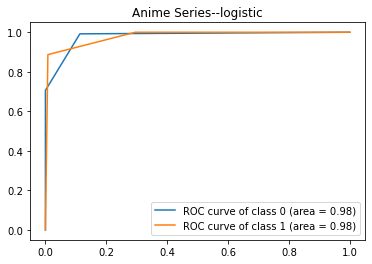
\includegraphics[width = 0.5 \textwidth]{ROCcurve/AnimeSeries_ROC.png}}
    \subfloat[\textit{Precission-Recall curve}]{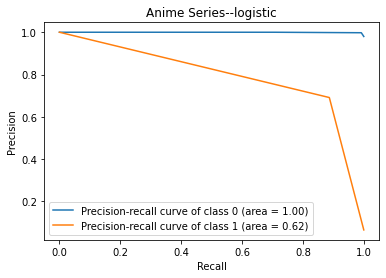
\includegraphics[width = 0.5 \textwidth]{PrecisionRecallCurve/AnimeSeries_RECALL.png}}
    \caption{Corba \textit{ROC} i \textit{Precission-Recall} del model Logístic per la variable \textit{Anime Series}}
    \label{fig:my_label}
\end{figure}\\
S'observa de les corbes ROC i Precission-Recall un resultat similar al obtingut amb la variable \textit{International TV Show}.\\
Es conclou doncs que té un bon resultat ja que les dues corves (ROC i Precission-Recall) obtenen valors propers a 1.
\newpage
\subsection{Precission-Recall i ROC curve del Random Forest}
\begin{figure}[h]
\centering
    \subfloat[\textit{ROC curve}]{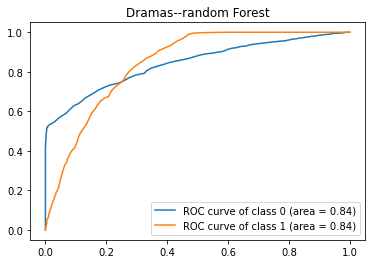
\includegraphics[width = 0.5 \textwidth]{ROCcurve/Dramas_ROC.png}}
    \subfloat[\textit{Precission-Recall curve}]{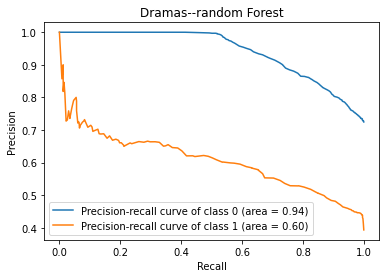
\includegraphics[width = 0.5 \textwidth]{PrecisionRecallCurve/Dramas_RECALL.png}}
    \caption{Corba \textit{ROC} i \textit{Precission-Recall} del Random Forest per la variable \textit{Dramas}}
    \label{fig:my_label}
\end{figure}
\hspace{-1.5em}S'observa, a partir de la corba ROC, com la sensitibitat del model és bona tot i que és pitjor que les que s'han obtingut en les variables objectius classificades amb els models logístic.\\\\
Per altra banda, preocupa la precissió del model, tal i com és pot observar en la corva Precission-Recall. El model tendeix a tenir problemes de precissió en la classificació de les produccions que tenen de gènere \textit{Dramas}. \\\\
Aquest comportament pot ser degut a la falta de dades i seria mitigat si es pogués introduïr-ne de més.\\\\
Tot i així, el model obté bones prediccion i té un bon resultat d'area sota la corba Precission-Recall que, segurament, seran millorats amb la implementació del millors hiperparàmetres.\\\\
Es conclou doncs que té un bon resultat ja que les dues corves (ROC i Precission-Recall) obtenen valors propers a 1.
\newpage 
\subsection{Precission-Recall i ROC curve de les Xarxes Neurals}
\begin{figure}[h]
\centering
    \subfloat[\textit{ROC curve}]{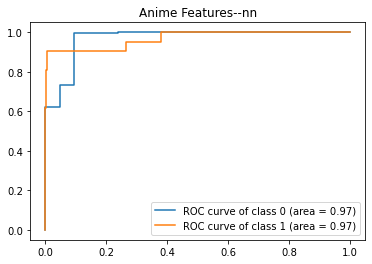
\includegraphics[width = 0.5 \textwidth]{ROCcurve/AnimeFeatures_ROC.png}}
    \subfloat[\textit{Precission-Recall curve}]{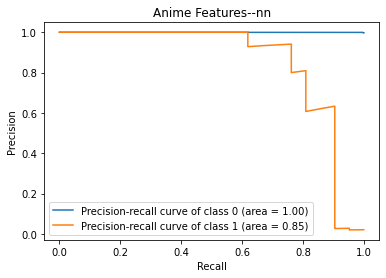
\includegraphics[width = 0.5 \textwidth]{PrecisionRecallCurve/AnimeFeatures_RECALL.png}}
    \caption{Corba \textit{ROC} i \textit{Precission-Recall} del model 3 de xarxa neural per la variable \textit{Anime Features}}
    \label{fig:my_label}
\end{figure}
\hspace{-1.5em}S'observa com el model de xarxa neural 3 és molt eficient a l'hora de classificar les produccions segons el gènere \textit{Anime Features}.\\\\
Els valors obtinguts tant en la corba ROC com Precission-Recall son molt propers a 1 o iguals, pel que reafirma la seva bona capacitat de classificació.
\\\\
Tot i així el classificador té problemes de precissió una vegada la recall supera el 0.8.\\\\
És Conclou que el model de xarxa neural 3 és un molt bon classificador.
\newpage 
\begin{figure}[h]
\centering
    \subfloat[\textit{ROC curve}]{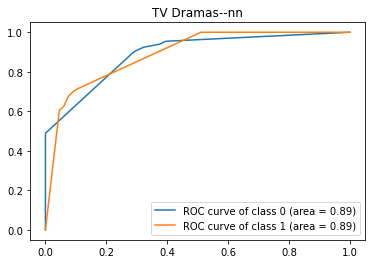
\includegraphics[width = 0.5 \textwidth]{ROCcurve/TVDramas_ROC.png}}
    \subfloat[\textit{Precission-Recall curve}]{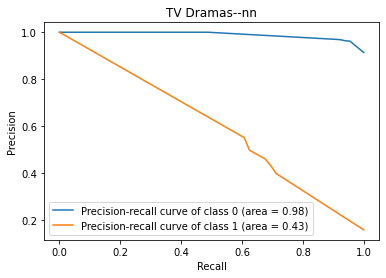
\includegraphics[width = 0.5 \textwidth]{PrecisionRecallCurve/TVDramas_RECALL.png}}
    \caption{Corba \textit{ROC} i \textit{Precission-Recall} del model 1 de xarxa neural per la variable \textit{TV Dramas}}
    \label{fig:my_label}
\end{figure}
\hspace{-1.5em}S'observa, com el model de xarxa neural 1 te problemes per classificar les produccions segons el gènere \textit{TV Drama}.\\\\
Enfatisar que aquest problemes son degut segurament a la falta de fiabilitat de les dades, ja que es tracten de les obtingudes pels mètodes que, ja de per si, obtenen certs errors.\\\\
Per altra banda, s'observa de les corbes ROC com té una bona sensitibitat, peró analitzant les corbes Precission-Recall és conslou que el model classifica pitjor que una classificació aleatória.\\\\
Recalcar que, tot i semblar que el model classifica erroniament, a la practica dona molt bons resultats, hi els resultats que obtenim en les corbes de Precission-Recall segurament son degudas a que hi existeixen poques produccions a la base de dades que tinguin gènere \textit{Drama}.\\\\
És conclou doncs que el model de xarxa neural 1 és bo tot i que s'espera millors resultats una vegada aplicada la cerca d'hiperparàmetres.
\newpage 
\section{Cerca d'hiperparàmetres}
\subsection{Hiperparàmetres dels models}
Exposem ara els millors hiperparàmetres per model i per atribut:
\begin{table}[h]
    \centering
    \begin{tabular}{c|c|c|c}
        \textbf{Model} & \textbf{Atributs} & \textbf{Hiperparàmetres} & \textbf{Precissió}  \\ \hline \hline
        \multirow{6}{*}{Logístic} & International TV & \multirow{6}{*}{\begin{tabular}{c}
            C: $K$  \\
            penalty: l2  \\
            solver: lbfgs \\
            random\_state: 0 \\
        \end{tabular}} & 0.95  \\
        & International Movies & & 0.94 \\
        & British TV & & 0.89\\
        & Spanish-Lan. TV & & 0.53\\
        & Anime Series & & 0.87\\
        & Korean TV & & 0.91\\\hline 
        \multirow{4}{*}{Random Forest} & \multirow{4}{*}{Dramas} & n\_estimators: 450 & \multirow{4}{*}{0.52}\\
        & & max\_features: $log_2(n)$& \\
        && criterion: entropy & \\
        && random\_state: 0 & \\ \hline 
        \multirow{14}{*}{Neural Network} & \multirow{7}{*}{Anime Features} & activation: relu& \multirow{7}{*}{0.81}\\
        && alpha: $\alpha_1$ &\\
        && learnung\_rate: constant &\\
        && learning\_rate\_init: $L_1$ &\\
        && solver: lbfgs &\\
        && random\_state: 0&\\
        && hidden\_layer\_sizes: (20, 20) &\\ \cline{2-4}
       & \multirow{7}{*}{TV Drama} & activation: identity & \multirow{7}{*}{0.60}\\
       && alpha: $\alpha_2$ &\\
        && learnung\_rate: invscaling &\\
        && learning\_rate\_init: $L_2$ &\\
        && solver: lbfgs &\\
        && random\_state: 0&\\
        && hidden\_layer\_sizes: (20,20) &\\
    \end{tabular}
    \caption{Taula amb els millors paràmetres de cada model per cada variable objectiu i la seva recall}
    \label{tab:my_label}
\end{table}
Recarcar que, els paràmetres que associem a constants $K, \alpha_1, \alpha_2, L_1$ i $L_2$ és per la gran quantitat de decimals que contenen les constants trobades. Concretament, valen:
\begin{itemize}
    \item $K= 2.5835764522666245$
    \item $\alpha_1= 0.6458941130666561$
    \item $\alpha_2= 0.02021839744032572$
    \item $L_1= 0.2975346065444723$
    \item $L_2= 0.7781567509498505$
\end{itemize}
Per altre banda, s'observa com la precissió augmenten/estabilitcen en valors més elevats que abans, pel que podem afirmar que la cerca d'hiperparàmetres ha funcionat correctament.\\\\
Analitcem ara les corbes ROC i Precission-Recall de cada model amb els hiperparàmetres.
\subsection{Resultats d'aplicar els hiperparàmetres}
\subsubsection{Precission-Recall i ROC curve dels models Logístics}
\begin{figure}[h]
\centering
    \subfloat[\textit{ROC curve}]{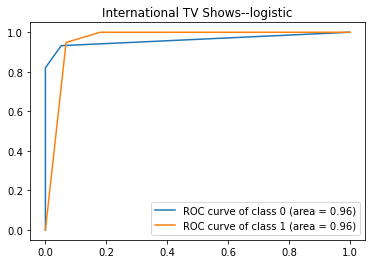
\includegraphics[width = 0.5 \textwidth]{BetterROC/BETTER_InternationalTV_ROC.png}}
    \subfloat[\textit{Precission-Recall curve}]{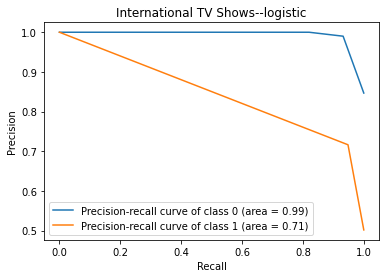
\includegraphics[width = 0.5 \textwidth]{BetterPrecision/BETTER_InternationalTV_RECALL.png}}
    \caption{Corba \textit{ROC} i \textit{Precission-Recall} del model Logístic per la variable \textit{International TV Shows}}
    \label{fig:my_label}
\end{figure}
\hspace{-1.5em}S'observa de les curves ROC que el model te una bona sensibilitat.\\\\
A més, la tendencia a perde recall ara és menys pronunciada pero perd recall abans; fent així que perdi valor d'area respecte abans de la cerca d'hiperparàmetres.\\\\
Tot i així te un bon resultat ja que les dues corves (ROC i Precission-Recall) obtenen valor propers a 1.\\
\begin{figure}[h]
\centering
    \subfloat[\textit{ROC curve}]{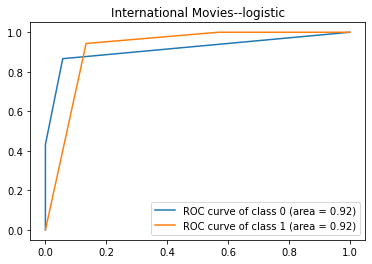
\includegraphics[width = 0.5 \textwidth]{BetterROC/BETTER_InternationalMovie_ROC.png}}
    \subfloat[\textit{Precission-Recall curve}]{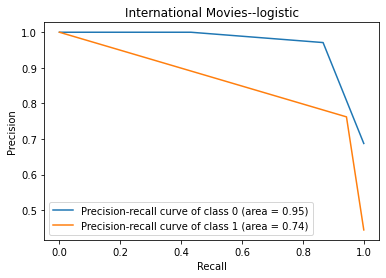
\includegraphics[width = 0.5 \textwidth]{BetterPrecision/BETTER_InternationalMovie_RECALL.png}}
    \caption{Corba \textit{ROC} i \textit{Precission-Recall} del model Logístic per la variable \textit{International TV Shows}}
    \label{fig:my_label}
\end{figure}\\
S'observa de les corbes ROC i Precission-Recall un resultat similar al obtingut amb la variable \textit{International TV Show}.\\
Es conclou doncs que té un bon resultat ja que les corves obtenen valors propers a 1.
\newpage
\begin{figure}[h]
\centering
    \subfloat[\textit{ROC curve}]{\includegraphics[width = 0.5 \textwidth]{BetterROC/BETTER_BritishTV_ROC.png}}
    \subfloat[\textit{Precission-Recall curve}]{\includegraphics[width = 0.5 \textwidth]{BetterPrecision/BETTER_BritishTV_RECALL.png}}
    \caption{Corba \textit{ROC} i \textit{Precission-Recall} del model Logístic per la variable \textit{British TV Shows}}
    \label{fig:my_label}
\end{figure}
\hspace{-1.5em}S'observa de les corbes ROC i Precission-Recall un resultat similar al obtingut amb la variable \textit{International TV Show}.\\
Es conclou doncs que té un bon resultat ja que les dues corves (ROC i Precission-Recall) obtenen valors propers a 1.\\
\begin{figure}[h]
\centering
    \subfloat[\textit{ROC curve}]{\includegraphics[width = 0.5 \textwidth]{BetterROC/BETTER_Spanish_ROC.png}}
    \subfloat[\textit{Precission-Recall curve}]{\includegraphics[width = 0.5 \textwidth]{BetterPrecision/BETTER_Spanish_RECALL.png}}
    \caption{Corba \textit{ROC} i \textit{Precission-Recall} del model Logístic per la variable \textit{Spanish-Language TV Shows}}
    \label{fig:my_label}
\end{figure}
S'observa com el model de classificació logístic te problemes per distingir si una producció és o no de gènere \textit{Spanish-Language TV Show}; tot i així, dona bons resultats quan s'utilitza i és basntant eficient.\\\\
També afegir, que els cambis en la forma de la corba ROC i Precission-Recall han sigut infims.\\\\
Es conclou doncs que té un resultat bo peró s'esperaba una millora més significativa.\\
\newpage 
\begin{figure}[h]
\centering
    \subfloat[\textit{ROC curve}]{\includegraphics[width = 0.5 \textwidth]{BetterROC/BETTER_Korean_ROC.png}}
    \subfloat[\textit{Precission-Recall curve}]{\includegraphics[width = 0.5 \textwidth]{BetterPrecision/BETTER_Korean_RECALL.png}}
    \caption{Corba \textit{ROC} i \textit{Precission-Recall} del model Logístic per la variable \textit{Korean TV Shows}}
    \label{fig:my_label}
\end{figure}
\hspace{-1.5em}S'observa de les corbes ROC i Precission-Recall un resultat similar al obtingut amb la variable \textit{International TV Show}.\\
Es conclou doncs que té un bon resultat ja que les dues corves (ROC i Precission-Recall) obtenen valors propers a 1.\\
\begin{figure}[h]
\centering
    \subfloat[\textit{ROC curve}]{\includegraphics[width = 0.5 \textwidth]{BetterROC/BETTER_AnimeSeries_ROC.png}}
    \subfloat[\textit{Precission-Recall curve}]{\includegraphics[width = 0.5 \textwidth]{BetterPrecision/BETTER_AnimeSeries_RECALL.png}}
    \caption{Corba \textit{ROC} i \textit{Precission-Recall} del model Logístic per la variable \textit{Anime Series}}
    \label{fig:my_label}
\end{figure}
S'observa de les corbes ROC i Precission-Recall un resultat similar al obtingut amb la variable \textit{International TV Show}.\\
Es conclou doncs que té un bon resultat ja que les dues corves (ROC i Precission-Recall) obtenen valors propers a 1.
\newpage
\begin{center}
    \textsc{\textbf{Comentari General sobre el model Logístic:}}
\end{center}
S'esperaba una millora més significativa en les corbes Precission-Recall una vegada optimitzats els hiperparàmetres.\\\\
Exposem les idees de que ha pogut succeir per a que obtingues les millores esperables:
\begin{itemize}
    \item El regressor ja, una vegada optimitzat, pot augmentar la seva precissió a l'hora de classificar, pero les caracteristiques entre la Precission i la Recall és manté constant.
    \item El mètode utilitzat\footnote{S'ha utilitzat, degut a la gran quantitat d'hiperparàmetres a cecar, el mètode \textit{RandomizedSearchCV} de la llibreria \textit{sklearn} } per a trobar la millor combinació d'hiperparàmetres no és el millor i ha donat una combinació d'hiperparàmetres que millora la precissió només en alguns casos.
\end{itemize}

\newpage
\subsubsection{Precission-Recall i ROC curve del Random Forest}
\begin{figure}[h]
\centering
    \subfloat[\textit{ROC curve}]{\includegraphics[width = 0.5 \textwidth]{BetterROC/BETTER_Drama_ROC.png}}
    \subfloat[\textit{Precission-Recall curve}]{\includegraphics[width = 0.5 \textwidth]{BetterPrecision/BETTER_Drama_RECALL.png}}
    \caption{Corba \textit{ROC} i \textit{Precission-Recall} del Random Forest per la variable \textit{Dramas}}
    \label{fig:my_label}
\end{figure}
\hspace{-1.5em}S'observa, a partir de la corba ROC, com la sensitibitat del model és bona tot i que és pitjor que les que s'han obtingut en les variables objectius classificades amb els models logístic.\\\\
Recarcar que, no ha patit grans cambis en la distribució/forma de les corbes ROC i Precission-Recall, pel que pot corroborar les hipótesis abans plantejades com a comentaris del model Logístic.\\\\
Tot i així, el model obté bones prediccion i té un bon resultat d'area sota la corba Precission-Recall.\\\\
Es conclou doncs que té un bon resultat ja que les dues corves (ROC i Precission-Recall) obtenen valors propers a 1.
\newpage 
\subsubsection{Precission-Recall i ROC curve de les Xarxes Neurals}
\begin{figure}[h]
\centering
    \subfloat[\textit{ROC curve}]{\includegraphics[width = 0.5 \textwidth]{BetterROC/BETTER_AnimeFeatures_ROC.png}}
    \subfloat[\textit{Precission-Recall curve}]{\includegraphics[width = 0.5 \textwidth]{BetterPrecision/BETTER_AnimeFeatures_RECALL.png}}
    \caption{Corba \textit{ROC} i \textit{Precission-Recall} de la xarxa neural per la variable \textit{Anime Features}}
    \label{fig:my_label}
\end{figure}
\hspace{-1.5em}S'observa com, ara si, les corves han cambiat respecte les obtingudes anteriorment. \\\\
De les corbes ROC corroborem que el model de xarxes neurals és bo per a la classificació de l'atribut \textit{Anime Features}. Per altra banda, les corbes de Precission-Recall indiquen que el classificador té problemes per d'obtenir bones Preccions i Recall a l'hora. \\\\
Aquesta diferencia de resultats respecte a les corbes Precission-Recall obtingudes pot ser deguda perque en aquest cas, s'ha repetir varies vegades l'experiment i ha mostrar que, si bé el model és bo classificant, no es tant bo com s'esperaba degut a possibles overfitting i processos de memorització del model.\\\\
És conclou que el model és prou bo. 
\newpage 
\begin{figure}[h]
\centering
    \subfloat[\textit{ROC curve}]{\includegraphics[width = 0.5 \textwidth]{BetterROC/BETTER_TVDrama_ROC.png}}
    \subfloat[\textit{Precission-Recall curve}]{\includegraphics[width = 0.5 \textwidth]{BetterPrecision/BETTER_TVDrama_RECALL.png}}
    \caption{Corba \textit{ROC} i \textit{Precission-Recall} de la xarxa neural per la variable \textit{TV Dramas}}
    \label{fig:my_label}
\end{figure}
\hspace{-1.5em}S'observa, com el model de xarxa neural no ha variat respecte el ja obtingut anteriorment. \\\\
Aquest efecte segurament és degut a que, com ja hem explicat anteriorment, no és pot augmentar més la precissió del model degut a les poques dades i la dependencia que té respecte als resultats obtinguts pels altres classificadors.\\\\
Tot així obté bons resultats pel que és conclou que és un bon classificador.  

\newpage 
\section{Conclusions}
Concluïm l'estudi mostrant les capacitats del classificador proposat, que esta format pels classificadors següents.
\begin{center} % 0.5-b-lbfgs-l2 0.8275
    \begin{tabular}{c|c|c|c|c|c|c}
        \multicolumn{2}{c|}{\textbf{Model}}  & \multicolumn{2}{c|}{\textbf{Temps d'execució (s)}} & \multirow{2}{*} {\textbf{Precission}} & \multirow{2}{*}{\textbf{Recall}} & \multirow{2}{*}{\textbf{Accuracy}} \\ 
        Clas. & Atribut & 30\% data & $25\cdot10^4$ prod. &  &  & \\ \hline\hline 
        \multirow{6}{*}{Logístic} & International TV & 0.01 & 0.02 & 0.72 & 0.95 & 0.82  \\ %0.72 0.95 0.82 0.01
        & International Mov. & 0.01 & 0.02 & 0.76 & 0.94 & 0.84   \\ % 0.76 0.94 0.84 0.01
        & British TV & 0.01 & 0.02 & 0.86 & 0.89 & 0.88 \\ %0.86 0.89 0.88 0.01
        & Spanish-Lan. TV & 0.01 &0.03& 0.74 & 0.54 & 0.62 \\ %0.74 0.54 0.62 0.01
        & Anime Series & 0.01 &0.02 & 0.69 & 0.89 & 0.78\\ %0.69 0.89 0.78 0.01
        & Korean TV & 0.01 &0.03 & 0.75 & 0.91 & 0.82 \\\hline %0.75 0.91 0.82 0.01
        Rnd Forest & Dramas & 1.11 &36.85& 0.59 & 0.52 & 0.55 \\ \hline 
        \multirow{2}{*}{NN} & Anime Features & 0.44 & 0.94  &0.74 & 0.81 & 0.77 \\ %0.74 0.81 0.77 0.44
        &TV Drama&  0.95 & 0.9 & 0.56 & 0.6 & 0.58\\ %0.56 0.6 0.58 0.95
        \end{tabular}
\label{tab:afins}
\end{center}
Recalcar, finalemnt, que aquest classificador (tot i ser el millor testejat) no pot classificar tot els 31 gèneres que disposa la base de dades degut a que no disposem de suficients dades de la resta de gèneres. Per a poder obtenir un millor classificador s'hauria d'introduïr més exemples de produccions de la resta de gèneres no classificats.
\end{document}
